%%%%%%%% ICML 2020 EXAMPLE LATEX SUBMISSION FILE %%%%%%%%%%%%%%%%%

\documentclass{article}

% Recommended, but optional, packages for figures and better typesetting:
\usepackage{microtype}
\usepackage{graphicx}
\usepackage{subfigure}
\usepackage{booktabs} % for professional tables
% \usepackage{icml2020} with \usepackage[nohyperref]{icml2020} above.
\usepackage{hyperref}
\newcommand{\theHalgorithm}{\arabic{algorithm}}

\usepackage[accepted]{icml2020}
\icmltitlerunning{Frequency Analysis of Multi-Electrode Mapping for Atrial Fibrillation driver}


\begin{document}

\twocolumn[
\icmltitle{Frequency Analysis of Multi-Electrode Mapping \\for Atrial Fibrillation driver
detection}

\icmlsetsymbol{equal}{*}

\begin{icmlauthorlist}
\icmlauthor{Alexander Zolotarev}{sk}
\icmlauthor{Batyrzhan Alikhanov}{sk}
\icmlauthor{Kirill Chertoganov}{sk}
\end{icmlauthorlist}

\icmlaffiliation{sk}{Skolkovo Institute of Science and Technology, Moscow, Russia}
\icmlcorrespondingauthor{Alexander Zolotarev}{Alexander.Zolotarev@skoltech.ru}

\icmlkeywords{Machine Learning, ICML}

\vskip 0.3in
]

\printAffiliationsAndNotice{}

\begin{abstract}
The destruction of atrial fibrillation drivers (or ablation) remains one of the best treatment for atrial fibrillation, however it is hard to define the driver location by electrode mapping. In this study we try to create the supervised classification driver vs non-driver model based on NIOM-validated ground-truth labels. The data of 7 atrial fibrillation episodes mapped simultaneously by NIOM and electrode mapping was used for Fourier spectra calculation. We tested several ML algorithms and ## neural network with different optimizators. The best f1-score is 0.826 for neural network with RMSProp optimizator trained on Fourier spectra, which confirms the possibility to separate correctly driver and non-driver recordings based on Fourier spectra.   
\end{abstract}

\section{Introduction}
\label{submission}
Atrial fibrillation (AF) is the most common cardiac arrhythmia and the leading cause of stroke in the world \cite{Calkins2017, Packer2019, Asad2019}. The mechanism of this disease remains unclear, but several experimental and clinical studies suggest that AF may be caused and maintained by spatially-stable, extra-pulmonary sources of repetitive rotational activity called reentrant AF drivers \cite{Haissaguerre2014, Hansen2015, Narayan2012}. Driver ablation can slow the rate of AF, convert it to atrial tachycardia, or terminate AF and restore sinus rhythm\cite{Hansen2016}. Unfortunately, clinical multi-electrode mapping (MEM) can record only the electrical signals from the surface and may not detect the transmural conduction within the 3-dimensional structure of the human atria \cite{DeGroot2016, Hansen2018}.

One potential solution to improve AF treatment is related to the widespread adoption of Machine Learning (ML) techniques. In line with the goals of our own study, ML was used to identify the location of computationally simulated reentrant AF drivers in-silico \cite{McGillivray2018}; however, many limitations have prevented translation of this work. Paramount among these limitations is the lack of a gold standard for AF driver detection in the clinical setting as clinical MEM is plagued by both false positives and false negatives \cite{Benharash2015, Hansen2018, Vijayakumar2016}. Without a gold standard for validation, it would be impossible to correctly annotate the ML training set. Thus, an urgent need exists to develop a validated ML algorithm to improve AF driver detection to increase the success of patient-specific AF ablation. 

Previous studies \cite{Hansen2015, Hansen2018, Zhao2017} have shown that these limitations in the visualization of reentrant AF drivers can be overcome in the ex-vivo human heart by high-resolution subsurface near-infrared optical mapping (NIOM) with submillimeter resolutions. We hypothesized that ML, verified by high-resolution NIOM, can efficiently distinguish MEM electrograms as originating from a reentrant AF driver or non-driver based on frequency features (e.g. the characteristics of the Fourier spectrum). Furthermore, since reentrant AF drivers cover an area greater than a single electrode, we explored if averaging the features across neighborhoods of electrodes could improve automated driver identification. 
The goal of our work is to create different frequency-based ML approaches, validated by the high-resolution NIOM modality, to separate MEM samples into reentrant AF driver vs non-driver classes.

\section{Algortithms and Models}
\label{submission}

\subsection{Explanted Human Hearts and Inclusion Criteria}

Deidentified, coded human hearts were obtained from The Ohio State University Cardiac Transplant team and LifeLine of Ohio in accordance with The Ohio State University Institutional Review Board. Only hearts with sustained AF in which NIOM activation mapping clearly identified localized AF drivers were included in this study.

\begin{figure}[ht]
\vskip 0.2in
\begin{center}
\centerline{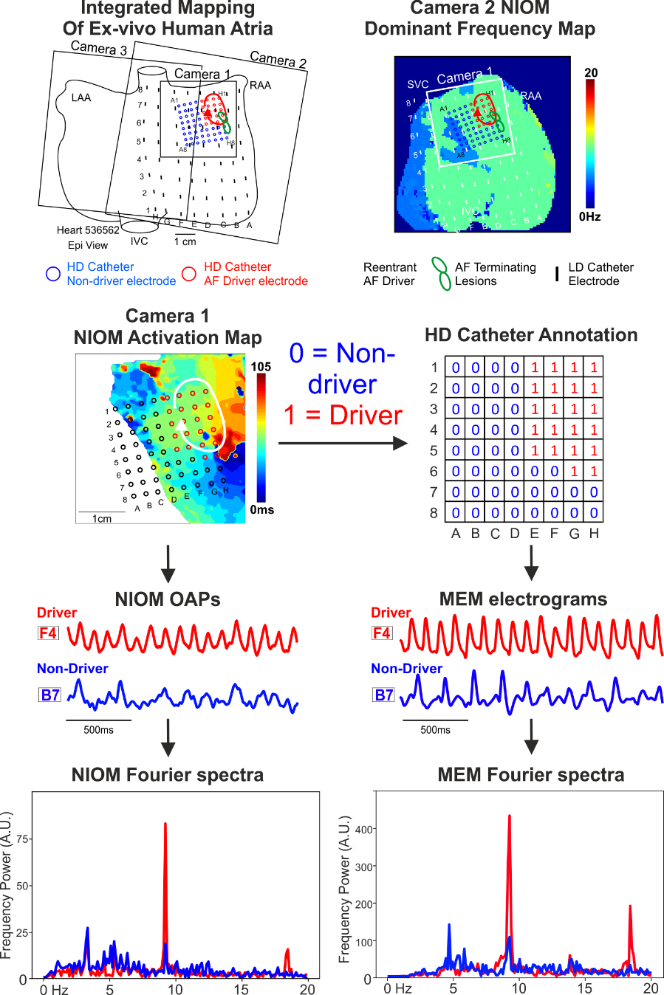
\includegraphics[width=\columnwidth]{image1.png}}
\caption{Analytical Pipeline for Driver Prediction.}
\label{icml-historical}
\end{center}
\vskip -0.2in
\end{figure}

Figure 1\footnote{LAA/RAA = Left/Right Atria Appendage, IVC = Inferior Vena Cava, MEM = Multi-Electrode Mapping, NIOM = Near-Infrared Optical Mapping, OAP = Optical Action Potential, A.U. = Arbitrary Units.} shows example of sustained AF episode maintained by reentrant driver, which was recorded simultaneously by clinical Higher-Density MEM catheter and high-resolution NIOM (Cameras 1-3). Ground-truth labels for electrodes (red – driver, blue – non-driver) were acquired by NIOM. Fourier spectra of annotated MEM electrograms and co-located NIOM OAPs were used for generation of frequency features for Machine Learning approach. 

\subsection{Multi-Electrode Mapping Electrograms}

For simultaneous NIOM and clinically-relevant MEM, 64-electrode (8x8) catheters with inter-electrode distance 3mm, 24mm x 24mm surface coverage, Higher Density [HD] flattened catheter \cite{Hansen2018a, Hansen2018} were provided by Abbott EP. The catheter grid was placed on the atrial tissue to cover the driver region indicated by the NIOM activation map (Figure 1).  Each recording was taken with the electrodes in a single position and point by point mapping was not used. Electrograms were recorded during the AF episodes simultaneously with NIOM optical action potentials (OAPs). The duration of the recordings varied from 8 to 16 seconds. 

\subsection{Data Annotation Workflow}

The ground truth for driver annotation  was the same as in prior studies \cite{Hansen2015, Hansen2018}. First, NIOM dominant frequency (DF, the frequency of the highest peak in the Fourier spectrum) was used to identify the fastest activating region, and then activation patterns based on the maximum derivative of NIOM optical action potentials are used to determined surface activation patterns within this region. The preferential driver activation paths were defined independently by three reviewers and electrodes within one ablation lesion distance (~5mm) of the paths were defined as driver center electrodes (class 1) and electrodes of outside of this distance threshold were defined as non-driver (class 0). Final reported annotation represent agreement among all three reviewers. Uninformative recordings (e.g., from electrodes with bad tissue contact) were annotated as outliers (class -1). A simultaneously recorded NIOM OAP was manually selected within less than 1 mm adjacent to each electrode location. By doing so, the recordings from the optical and the electrode mapping modalities were guaranteed to be co-located for further correlation and ML-based analysis.

\begin{figure}[ht]
\vskip 0.2in
\begin{center}
\centerline{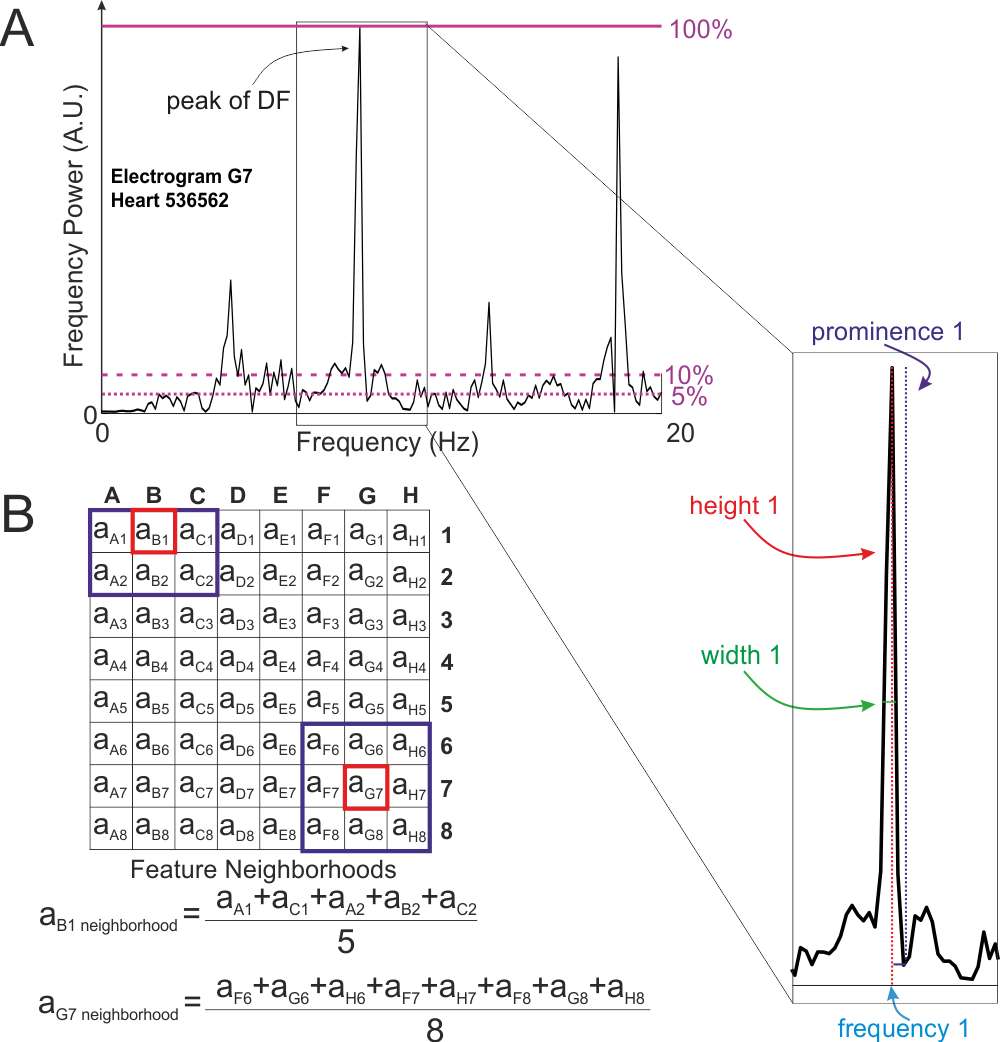
\includegraphics[width=\columnwidth]{image3.png}}
\caption{Analytical Pipeline for Driver Prediction.}
\label{icml-historical}
\end{center}
\vskip -0.2in
\end{figure}

\subsection{Raw Signal Preprocessing}

We applied signal normalization and 2-20 Hz Butterworth band-pass filtering to all recordings. MEM recordings were then resampled into 5 second segments by a sliding window with 0.5 second steps (for Short-Time Fourier Transformation). Fourier spectra were then calculated for each 5 second recording using a Fast Fourier Transform from NumPy library in Python (https://numpy.org/).

A set of frequency features for training a ML model was then generated from each Fourier spectrum. The integer number n in the feature’s name corresponds to the number of the nth highest peak in the Fourier spectrum, ranging from the n = 1 peak (the peak of dominant frequency) to the n = 5 (the fifth highest peak). Spectral features height, width, frequency, and prominence, for each of the five highest peaks, were calculated using scipy.signal library in Python. An example of MEM spectrum and the aforementioned features are shown in Figure 2A. Features \#peaks\_0.05 and \#peaks\_0.1 correspond to the number of peaks higher than a given threshold (we chose 5\% and 10\% of the height of the dominant frequency peak, respectively) to reflect values of noise present in the recordings. The peak-to-standard deviation ratio (PSDR) feature was calculated as the ratio between the average height of the two highest peaks to the standard deviation of heights across the whole spectrum. The other features are the ratios between features for each of the five tallest peaks. 

For a given feature, each “Neighborhood” feature was then generated as a mean of the feature values of the 8 adjacent electrodes in a 3x3 grid, as visualized in Figure 2B. Total number of generated features is equal to 35. 

\subsection{Algorithm Selection and Testing}
We tested 4 ML classification algorithms: k-Nearest Neighbors (kNN), Support Vector Machine (SVM), Scalable Gradient Boosting (XGBoost), and Random Forest (RF). The hyperparameters were selected by SearchGrid for each algorithm. The training/testing sets were randomly obtained from a 70\%/30\% split of the dataset, with each set having been stratified to provide the same balance of driver and non-driver recordings. Importantly, the windows from one recording are located in either training or testing set to reduce experimental bias. Standard deviations reported herein were obtained by averaging the output of algorithms on 10-folds of the testing set. 

11 configurations of neural networks with different layers  (1,2,3,4,5,8,10,22,24,27,32) were tested, and it was discovered that best configuration was with 4 layers: 4 Linear layers, 4 Batchnorm,  4 RELU activation function, dropout=0.1. We tried to compare different optimizers between each other such as: RMSprop, SGD, Rprop, Adam. Better score was with RMSproop. Also we tried to play with different variants of dropout (0;0.05;0,1;0.2;0.5) and the best was dropout 0.1 it gaved better results: accuracy 0.892, precision 0.844, recall 0.8095,
f1 score: 0.826.

\subsection{Performance Metrics}

We used accuracy, precision, recall, f1-score and, area under the curve (AUC) for receiver operating characteristic (ROC) for each ML classification algorithm to evaluate its performance. ROC curve was used to select the best threshold for the binary classification between driver and non-driver recordings. The threshold was chosen to provide the best balance between recall and precision, and the best f1-score.

We investigated which features are the most valuable for the classification and how few features can be used without suffering a loss in f1-score. The subordinate features were removed until value of f1-score dropped below the original confidence interval. 

To carry out the feature importance analysis, we used an integrated feature\_importance function from the XGBoost library. The results were sorted in the descending order, with the most valuable feature being listed first and the relative contribution of the other features being normalized to the most valuable one.

\subsection{Statistical Analysis}
Metrics are presented as mean ± standard deviation, calculated on 10 folds of the testing set. The analysis was done using the scipy.stats library in Python. Statistical significance between metrics on different options of feature sets for the same dataset or between metrics on different datasets was analyzed by Tukey’s range test for pairwise samples, with the p-value < 0.05 being considered as significant. The assumption of the metrics to be sampled from the normal distribution was verified using the Shapiro-Wilk test. 
\section{Experiments and Results}
\label{submission}

\subsection{Samples}
The final dataset consisted of 7 reentrant AF episodes to test the ability of ML algorithm to distinguish driver recordings simultaneously mapped by MEM and. Each episode was mapped by 64-electrode grid, which resulted in total number 7 x 64 = 448 AF recordings. We expanded this number using data augmentation by Fourier transformation of window slices of AF recordings which is widely used in the field \cite{Cui2016, LeGuennec2016}. 

\begin{figure}[ht]
\vskip 0.2in
\begin{center}
\centerline{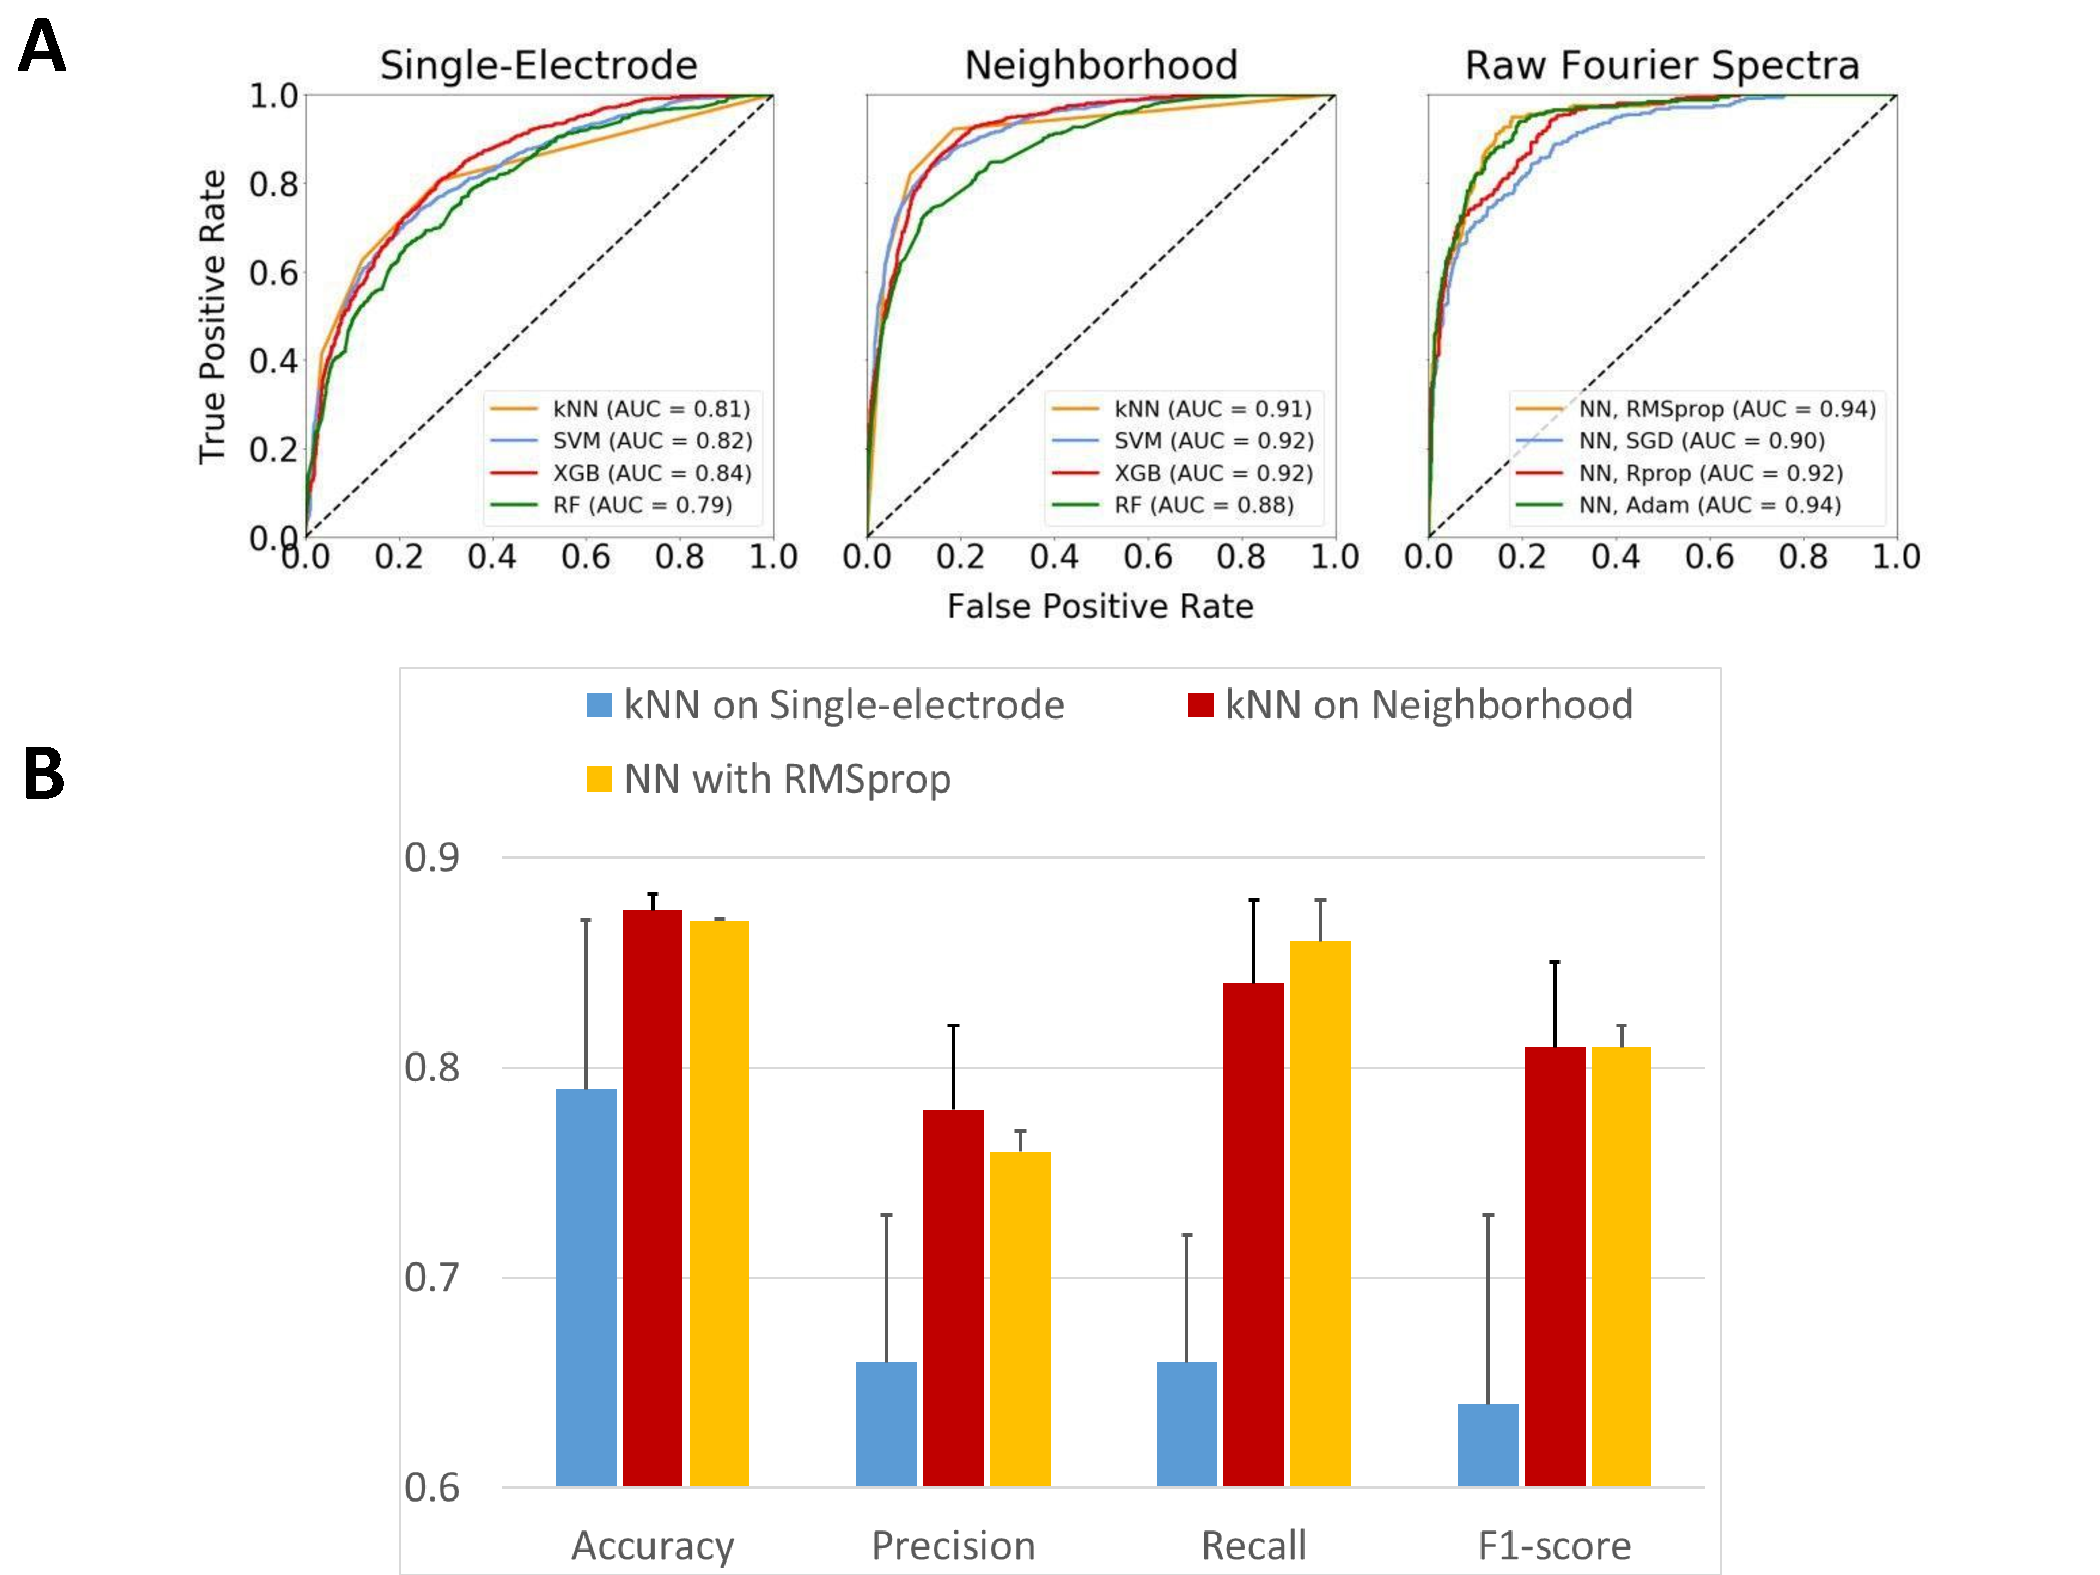
\includegraphics[width=\columnwidth]{image5.pdf}}
\caption{Performance of Binary Classification. (A) - The Receiver Operating Characteristic curves for different feature sets of AF dataset as analyzed by 4 algorithms. (B) - Performance metrics of kNN binary classification into AF reentrant driver vs non-driver recordings for different feature sets.}
\label{icml-historical}
\end{center}
\vskip -0.2in
\end{figure}

\subsection{Driver vs Non-Driver Classification}
Amongst the three frequency feature sets tested with the ML algorithm to classify MEM: single-electrode MEM features (n = 35 features), electrode-neighborhood MEM features (n = 35 features); neighborhood electrodes were the best performing. The ROC curves of the 4 ML algorithms considered (kNN, SVM, XGBoost, and RF) are shown in Figure 3A\footnote{MEM = Multi-Electrode Mapping, NIOM = Near-Infrared Optical Mapping. AUC = Area Under the Curve, kNN = k-Nearest Neighbors, SVM = Support Vector Machine, RF = Random Forest, XGB = XGBoost Classifier.}. kNN accounting for 3 neighbors proved to be the most efficient ML algorithm for the LD+HD dataset, with the number of optimal neighbors being equal to 3 and with a classification threshold of 0.5. The performance metrics (accuracy, precision, recall, and f1-score) for the different feature sets with the kNN model are presented in Figure 3B. 

Performance of driver classification could be improved by averaging the features of eight surrounding neighborhood electrodes. Figure 3B shows that the values of metrics for the electrode-neighborhood feature set are all significantly higher than those for the single-electrode feature set. Full report on the metrics predicted by the 4 ML algorithms can be found in Table 1. The most valuable features are listed in Figure 4. 

\begin{table}[t]
\caption{Statistical performance metrics for ML methods.}
\label{sample-table}
\vskip 0.15in
\begin{center}
\begin{small}
\begin{sc}
% \begin{tabular}{lcccr}
\begin{tabular}{l{1cm}p{2cm}p{2cm}r{2cm}}
\toprule
Model &Metrics &1 Electrode &Neighborhood\\
\midrule
KNN        &accuracy  &0.77 $\pm$ 0.09& 0.87 $\pm$ 0.01\\
&precision &0.63 $\pm$ 0.21 &0.78 $\pm$ 0.03\\
&recall    &0.65 $\pm$ 0.24 &0.84 $\pm$ 0.04\\
&f1        &0.63 $\pm$ 0.21 &0.81 $\pm$ 0.02\\\\

XGB    &accuracy  &0.71 $\pm$ 0.06 &0.81 $\pm$ 0.01\\
&precision &0.54 $\pm$ 0.1  &0.64 $\pm$ 0.02\\
&recall    &0.75 $\pm$ 0.15 &0.94 $\pm$ 0.02\\
&f1        &0.62 $\pm$ 0.10 &0.76 $\pm$ 0.02\\\\

RF         &accuracy  &0.68 $\pm$ 0.08 &0.83 $\pm$ 0.02\\
&precision &0.5  $\pm$ 0.12 &0.71 $\pm$ 0.03\\
&recall    &0.77 $\pm$ 0.2  &0.84 $\pm$ 0.03\\
&f1        &0.60 $\pm$ 0.13 &0.77 $\pm$ 0.03\\\\

SVM        &accuracy  &0.78 $\pm$ 0.07 &0.86 $\pm$ 0.01\\
&precision &0.66 $\pm$ 0.17 &0.80 $\pm$ 0.02\\
&recall    &0.66 $\pm$ 0.26 &0.77 $\pm$ 0.03\\
&f1        &0.64 $\pm$ 0.19 &0.78 $\pm$ 0.02\\\\

\toprule
Model & Metrics && initial Fourier spectra\\
\midrule
NN        &accuracy  &&0.89 $\pm$ 0.01\\
&precision &&0.84 $\pm$ 0.01\\
&recall    &&0.81 $\pm$ 0.02\\
&f1        &&0.826 $\pm$ 0.02\\\\
\bottomrule
\end{tabular}
\end{sc}
\end{small}
\end{center}
\vskip -0.1in
\end{table}

11 Neural Network architectures were tested with different parameter 
configuration. The hyperparameters were selected manually. The training/testing sets were randomly obtained
from a 70\%/30\% split of the dataset, with each set having
been stratified to provide the same balance of driver and
non-driver recordings. Standard deviations reported herein
were obtained by averaging the output of neural networks on
10-folds of the testing set.  Full report on the metrics predicted by the 4 layer deep learning neural network architecture with RMSprop optimizer can be found in Table 1. 
Link to github repo: \textbf{https://github.com/DersUzala/ML2020-project-of-group-33}

\begin{figure}[ht]
\vskip 0.2in
\begin{center}
\centerline{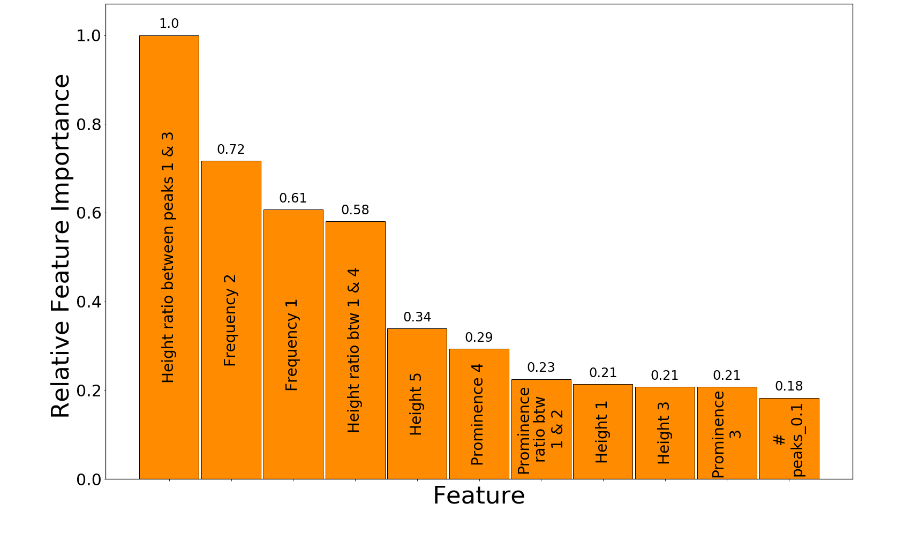
\includegraphics[width=\columnwidth]{image4.png}}
\caption{The most valuable features for AF HD MEM feature set.}
\label{icml-historical}
\end{center}
\vskip -0.2in
\end{figure}

% \begin{table}[t]
% \caption{Statistical performance metrics for NN.}
% \label{sample-table}
% \vskip 0.15in
% \begin{center}
% \begin{small}
% \begin{sc}
% % \begin{tabular}{lccr}
% \begin{tabular}{l{1cm}p{2cm}r{2cm}}
% \toprule
% Model & Metrics & initial Fourier spectra\\
% \midrule
% NN        &accuracy  &0.89 $\pm$ 0.01\\
% &precision &0.84 $\pm$ 0.01\\
% &recall    &0.81 $\pm$ 0.02\\
% &f1        &0.826 $\pm$ 0.02\\\\

% \bottomrule
% \end{tabular}
% \end{sc}
% \end{small}
% \end{center}
% \vskip -0.1in
% \end{table}

\section{CONCLUSION}

This pilot study has shown for the first time that a ML-based approach validated by high-resolution NIOM in human hearts could efficiently classify MEM electrograms into AF driver or non-driver recordings by using the features from the Fourier spectra. This approach performed better when considering features from electrogram neighborhoods instead of single electrograms. Further validation and training of the ML- approach by NIOM would improve future application as a complementary tool during clinical AF ablation procedures, bringing essential enhancement to the conventional clinical MEM approaches to detect AF drivers. 

% In the unusual situation where you want a paper to appear in the
% references without citing it in the main text, use \nocite
\nocite{langley00}

\bibliography{example_paper}
\bibliographystyle{icml2020}


%%%%%%%%%%%%%%%%%%%%%%%%%%%%%%%%%%%%%%%%%%%%%%%%%%%%%%%%%%%%%%%%%%%%%%%%%%%%%%%
%%%%%%%%%%%%%%%%%%%%%%%%%%%%%%%%%%%%%%%%%%%%%%%%%%%%%%%%%%%%%%%%%%%%%%%%%%%%%%%
%%%%%%%%%%%%%%%%%%%%%%%%%%%%%%%%%%%%%%%%%%%%%%%%%%%%%%%%%%%%%%%%%%%%%%%%%%%%%%%
%%%%%%%%%%%%%%%%%%%%%%%%%%%%%%%%%%%%%%%%%%%%%%%%%%%%%%%%%%%%%%%%%%%%%%%%%%%%%%%
\newpage
\clearpage
\appendix
\section{Team member's contributions}
\label{appendix-contrib}
Explicitly stated contributions of each team member to the final project.
\subsection*{Alexander Zolotarev (50\% of work)}
\begin{itemize}
    \item Reviewing literature on the topic
    \item Preprocessing the raw data into Fourier Spectra
    \item Feature Generation from Fourier Spectra
    \item Coding and experimenting with ML methods
    \item Preparing the GitHub Repo
    \item Preparing and recording the presentation
\end{itemize}

\subsection*{Batyrzhan Alikhanov (25\% of work)}
\begin{itemize}
    \item Literature Review
    \item Preprocessing the Fourier Spectra
    \item Development and experiments on NN architectures
    \item Preparing the report in LateX
\end{itemize}

\subsection*{Kirill Chertoganov (25\% of work)}
\begin{itemize}
    \item Literature Review
    \item Development and experiments on NN architectures
    \item Preparing the report in LateX 
    \item Preparing the presentation
\end{itemize}

\clearpage
\section{Reproducibility checklist}
\label{appendix-checklist}
Answer the questions of following reproducibility checklist. If necessary, you may leave a comment.
    \begin{enumerate}
    \item A ready code was used in this project, e.g. for replication project the code from the corresponding paper was used.
    \begin{itemize}
        \item [\faCheckSquareO] Yes.
        \item [\faSquareO] \textbf{\underline{No.}}
        \item [\faSquareO] Not applicable.
    \end{itemize}
    
    \textbf{General comment:} If the answer is \textbf{yes}, students must \underline{explicitly clarify} to which extent (e.g. which percentage of your code did you write on your own?) and which code was used.
    
    \textbf{Students' comment:} None
    \item A clear description of the mathematical setting, algorithm, and/or model is included in the report.
    \begin{itemize}
        \item [\faSquareO] \textbf{\underline{Yes.}}
        \item [\faSquareO] No.
        \item [\faSquareO] Not applicable.
    \end{itemize}
    
    \textbf{Students' comment:} None
    
    \item A link to a downloadable source code, with specification of all dependencies, including external libraries is included in the report.
    \begin{itemize}
        \item [\faSquareO] \textbf{\underline{Yes.}}
        \item [\faSquareO] No.
        \item [\faSquareO] Not applicable.
    \end{itemize}
    
    \textbf{Students' comment:} None
    
    \item A complete description of the data collection process, including sample size, is included in the report.
    \begin{itemize}
        \item [\faSquareO] \textbf{\underline{Yes.}}
        \item [\faSquareO] No.
        \item [\faSquareO] Not applicable.
    \end{itemize}
    
    \textbf{Students' comment:} None
    
    \item A link to a downloadable version of the dataset or simulation environment is included in the report.
    \begin{itemize}
        \item [\faSquareO] \textbf{\underline{Yes.}}
        \item [\faSquareO] No.
        \item [\faSquareO] Not applicable.
    \end{itemize}
    
    \textbf{Students' comment:} None
    
    \item An explanation of any data that were excluded, description of any pre-processing step are included in the report.
    \begin{itemize}
        \item [\faSquareO] \textbf{\underline{Yes.}}
        \item [\faSquareO] No.
        \item [\faSquareO] Not applicable.
    \end{itemize}
    
    \textbf{Students' comment:} None
    
    \item An explanation of how samples were allocated for training, validation and testing is included in the report.
    \begin{itemize}
        \item [\faSquareO] \textbf{\underline{Yes.}}
        \item [\faSquareO] No.
        \item [\faSquareO] Not applicable.
    \end{itemize}
    
    \textbf{Students' comment:} None
    
    \item The range of hyper-parameters considered, method to select the best hyper-parameter
configuration, and specification of all hyper-parameters used to generate results are included in the report.
    \begin{itemize}
        \item [\faSquareO] \textbf{\underline{Yes.}}
        \item [\faSquareO] No.
        \item [\faSquareO] Not applicable.
    \end{itemize}
    
    \textbf{Students' comment:} None
    
    \item The exact number of evaluation runs is included.
    \begin{itemize}
        \item [\faSquareO] \textbf{\underline{Yes.}}
        \item [\faSquareO] No.
        \item [\faSquareO] Not applicable.
    \end{itemize}
    
    \textbf{Students' comment:} None
    
    \item A description of how experiments have been conducted is included.
    \begin{itemize}
        \item [\faSquareO] \textbf{\underline{Yes.}}
        \item [\faSquareO] No.
        \item [\faSquareO] Not applicable.
    \end{itemize}
    
    \textbf{Students' comment:} None
    
    \item A clear definition of the specific measure or statistics used to report results is included in the report.
    \begin{itemize}
        \item [\faSquareO] \textbf{\underline{Yes.}}
        \item [\faSquareO] No.
        \item [\faSquareO] Not applicable.
    \end{itemize}
    
    \textbf{Students' comment:} None
    
    \item Clearly defined error bars are included in the report.
    \begin{itemize}
        \item [\faSquareO] \textbf{\underline{Yes.}}
        \item [\faSquareO] No.
        \item [\faSquareO] Not applicable.
    \end{itemize}
    
    \textbf{Students' comment:} None
    
    \item A description of the computing infrastructure used is included in the report.
    \begin{itemize}
        \item [\faSquareO] Yes.
        \item [\faSquareO] \textbf{\underline{No.}}
        \item [\faSquareO] Not applicable.
    \end{itemize}
    
    \textbf{Students' comment:} None
\end{enumerate}

\end{document}

